\section{Introducci\'on}
El trabajo expuesto en este documento tiene como fin la implantación de un museo virtual en el Observatorio de Madrid. La parte más importante en este tipo de proyectos (y, por extensión, de todos) es la recogida de requisitos y el análisis (en este caso, elección principalmente).
Para poder entender mejor lo que se solicita por parte del cliente es necesario conocer el concepto de "museo virtual" al que tratamos de acercarnos. Se trataría de una plataforma accesible físicamente desde puestos instalados en una sala de exposiciones dentro del propio observatorio, accesible en línea desde Internet y que comprenda una base de datos posiblemente reutilizable en el futuro. Con estas pinceladas he deducido que la solución existente (no hay que olvidar que esto es ingeniería) más cercana a lo que se nos pide pasaría, en mi opinión, por un gestor de contenidos o CMS (Content Management System).
Dada la amplísima oferta que hay de estos productos en el mercado, creo conveniente hacer una selección a partir de criterios, unos surgidos y otros sugeridos, analizados mano a mano con el cliente.
Como ob
Esta seccin representa una introduccin al Trabajo Fin de Carrera desarrollado.
a) Introducción en la que se indique el planteamiento del trabajo y los
objetivos a conseguir.
b) Base teórica en la que se expongan los conceptos teóricos utilizados para
la realización del trabajo, así como los cálculos realizados.
c) Descripción experimental, cuando sea necesario, descripción del diseño,
resultados, etc.
d) Conclusiones y futuro trabajo.


\subsection{Estado del Arte}
En el estado del arte se enumeran los trabajos ms relevantes de otros grupos de investigacin. A continuacin se muestra un ejemplo del uso de vietas que nos proporciona ''itemize'':

\begin{itemize}
\item En el trabajo ..... 
\item En el siguiente trabajo.....
\end{itemize}

Existen mltiples formas de insertar figuras en Latex. A continuacin, se muestra un ejemplo del uso de ''figure''. Como se puede ver en la Figura \ref{fig1} tambin se pueden poner referencias a las figuras por medio de ''ref'' y la etiqueta ''label'' de la figura en particular.

\begin{figure}[h] %el especificador [h] indica que ponga la figura aqui si es posible
\centering
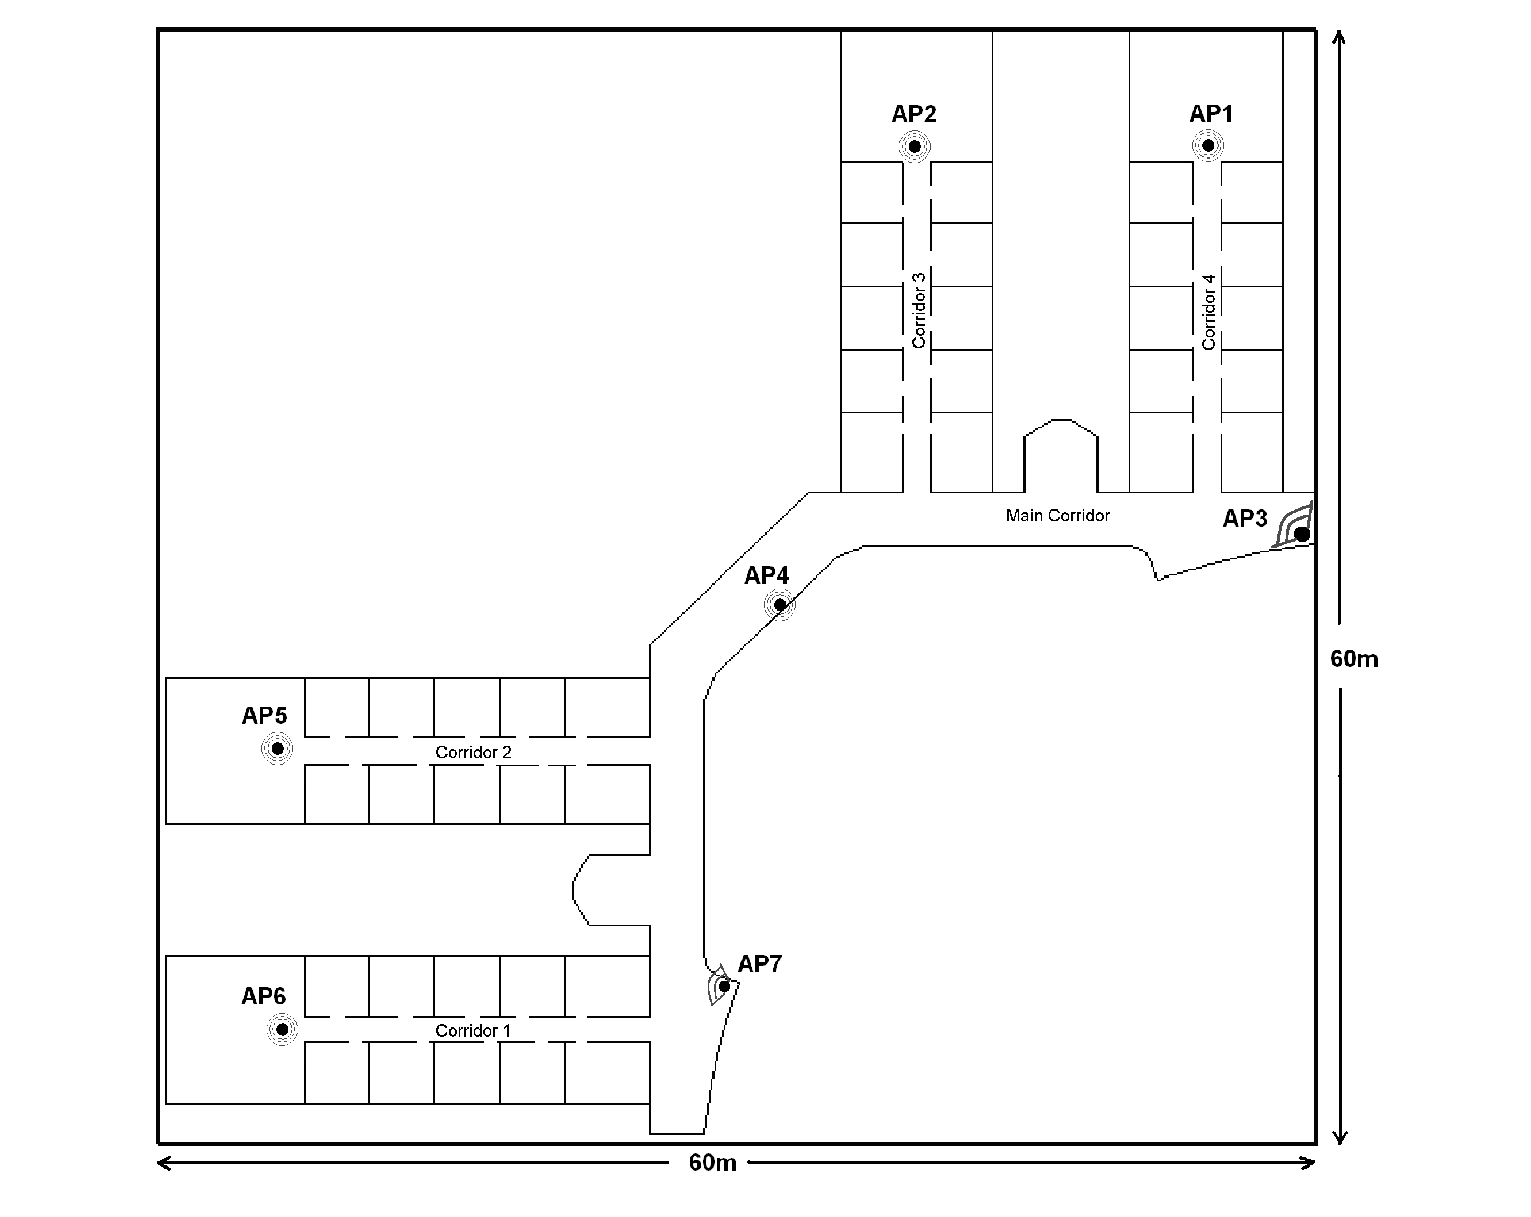
\includegraphics[width=4.7in]{Figure1.eps}
% where an .eps filename suffix will be assumed under latex, 
% and a .pdf suffix will be assumed for pdflatex
\caption{Departmento de Electr\'onica}
\label{fig1}
\end{figure}



\subsection{Objetivos}

Los objetivos principales de este Trabajo Fin de Carrera son (ejemplo utilizando ''enumerate''):

\begin{enumerate}
\item Primer objetivo ..... 
\item Segundo objetivo.....
  \begin{enumerate}
  \item Objetivo 2.1....
  \item Objetivo 2.2....
  \end{enumerate}
\item Tercer objetivo....
\end{enumerate}

\section{Desarrollo}

En esta seccin se incluir el desarrollo del trabajo.

Tambin resulta til poder introducir ecuaciones que se encuentran tanto en lnea con el texto $\sigma=0.75$, como en un prrafo aparte (ver ecuacin \ref{eq1}). Al igual que ocurre con las figuras, tambin se pueden referenciar las ecuaciones. 


\begin{equation}
  p[q_t=\sigma_t|q_{t-1}=\sigma_{t-1}]\label{eq1}
\end{equation}



\section{Resultados}
En este apartado se introducirn los resultados ms relevantes del trabajo.

A continuacin, se muestra un ejemplo de tabla simple (ver tabla \ref{table1}).

\begin{table}
  % increase table row spacing, adjust to taste
  \renewcommand{\arraystretch}{1.3}
  \caption{Comparativa}
  \label{table1}
  \begin{center}
    % Some packages, such as MDW tools, offer better commands for making tables
    % than the plain LaTeX2e tabular which is used here.
    \begin{tabular}{|c|c|c|}
      \hline
      Method & Training Time & Man-Work (\%)\\
      \hline
      Propagation model & $<$ 30 sec & 5\\
      \hline
      Manual & 9 h 30 min & 24\\
      \hline
      Automatic & 2 h & 10 8\\
      \hline
    \end{tabular}
  \end{center}
\end{table}

Cuando las tablas ocupan ms de un pgina se debe utilizar un tipo especial de tablas denominado ''longtbale''. A continuacin, se muestra un ejemplo del mismo (ver tabla \ref{table2}).

\begin{center}
	\begin{longtable}{|c|c|c|c|}
	\caption[Resultados de la Correlacion cruzada]{Resultados de la Correlacin cruzada} \label{table2} \\
	
	\hline \multicolumn{1}{|c|}{\textbf{Posicin Real}} & \multicolumn{1}{c|}{\textbf{Posicin estimada}} & \multicolumn{1}{c|}{\textbf{Coef. Correlacin}} & \multicolumn{1}{c|}{\textbf{Acierto/Fallo}} \\ \hline 
	\endfirsthead
	
	\multicolumn{4}{c}%
	{{\bfseries \tablename\ \thetable{} -- continua en la pgina anterior}} \\
	\hline \multicolumn{1}{|c|}{\textbf{Posicin Real}} & \multicolumn{1}{c|}{\textbf{Posicin estimada}} & \multicolumn{1}{c|}{\textbf{Coef. Correlacin}} & \multicolumn{1}{c|}{\textbf{Acierto/Fallo}} \\ \hline 
	\endhead
	
	\hline \multicolumn{4}{|r|}{{Continua en la pgina siguiente}} \\ \hline
	\endfoot
	\hline \hline
	\endlastfoot
	
	\hline	2P0	&	2P0	&	0,004954	&	A	\\
	\hline	2P1	&	2P4	&	0,005752	&	F	\\
	\hline	2P2	&	2P2	&	0,005461	&	A	\\
	\hline	2P3	&	2P0	&	0,004634	&	F	\\
	\hline	2P5	&	2P4	&	0,005991	&	F	\\
	\hline	2P6	&	2P16	&	0,004410	&	F	\\
	\hline	2P7	&	3P9	&	0,008038	&	F	\\
	\hline	2P8	&	3P9	&	0,003753	&	F	\\
	\hline	2P9	&	2P7	&	0,004908	&	F	\\
	\hline	2P10	&	2P10	&	0,007273	&	A	\\
	\hline	2P14	&	2P16	&	0,006485	&	F	\\
	\hline	2P15	&	2P15	&	0,004932	&	A	\\
	\hline	2P16	&	2P16	&	0,006237	&	A	\\
	\hline	2P17	&	2P15	&	0,005110	&	F	\\
	\hline	2P18	&	3P18	&	0,006235	&	F	\\
	\hline	2P19	&	3P18	&	0,004827	&	F	\\
	\hline	2P20	&	2P20	&	0,006877	&	A	\\
	\hline	2P22	&	3P18	&	0,003048	&	F	\\
	\hline	2P24	&	2P24	&	0,006833	&	A	\\
	\hline	2P25	&	2P25	&	0,004875	&	A	\\
	\hline	2P26	&	2P31	&	0,005511	&	F	\\
	\hline	2P27	&	2P28	&	0,004590	&	F	\\
	\hline	2P30	&	2P31	&	0,005576	&	F	\\
	\hline	2P31	&	2P31	&	0,007213	&	A	\\
	\hline	2P32	&	2P35	&	0,003340	&	F	\\
	\hline	2P34	&	2P34	&	0,004128	&	A	\\
	\hline	2P36	&	2P35	&	0,003329	&	F	\\
	\hline	2P37	&	2P37	&	0,003468	&	A	\\
	\hline	2P39	&	2P38	&	0,002577	&	F	\\
	\hline	2P40	&	2P43	&	0,004303	&	F	\\
	\hline	2P41	&	2P41	&	0,001573	&	A	\\
	\hline	2P42	&	2P41	&	0,000846	&	F	\\
	\hline	2P44	&	2P44	&	0,002732	&	A	\\
	\hline	2P45	&	23P45	&	0,001958	&	F	\\
	\hline	2P47	&	2P34	&	0,002869	&	F	\\
	\hline	2P48	&	2P43	&	0,004569	&	F	\\
	\hline	2P49	&	3P51	&	0,001374	&	F	\\
	\hline	2P50	&	2P34	&	0,002274	&	F	\\
	\hline	2P51	&	2P63	&	0,003931	&	F	\\
	\hline	2P52	&	2P55	&	0,003537	&	F	\\
	\hline	2P53	&	3P56	&	0,003126	&	F	\\
	\hline	2P54	&	2P67	&	0,005560	&	F	\\
	\hline	2P56	&	2P55	&	0,002817	&	F	\\
	\hline	2P57	&	2P67	&	0,006168	&	F	\\
	\hline	2P58	&	2P58	&	0,005278	&	A	\\
	\hline	2P60	&	3P66	&	0,004966	&	F	\\
	\hline	2P61	&	3P61	&	0,004748	&	A	\\
	\hline	2P64	&	2P67	&	0,005342	&	F	\\
	\hline	2P66	&	2P4	&	0,004172	&	F	\\
	\hline	2P67	&	2P67	&	0,005706	&	A	\\
	\hline	3P0	&	3P0	&	0,003674	&	A	\\
	\hline	3P61	&	2P61	&	0,003263	&	F	\\
	\hline	3P64	&	2P67	&	0,003484	&	F	\\
	\hline	3P65	&	2P67	&	0,002975	&	F	\\
	\hline	3P66	&	2P58	&	0,005029	&	F	\\
	\hline	3P67	&	3P67	&	0,003714	&	A	\\
	\end{longtable}
	\end{center}



En algunas ocasiones, también resulta útil emplear el entorno ''subfigure'' para añadir múltiples imágenes dentro de la misma figura. A continuación, se muestra un ejemplo del uso en la figura \ref{fig2}. También se pueden referenciar las sub-figuras de forma individual, por ejemplo la sub-figura \ref{fig2b}.

\begin{figure}[h]
\centerline{\subfigure[Mean entropy]{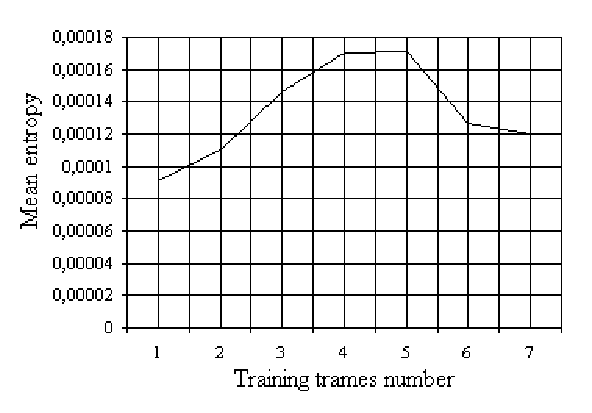
\includegraphics[width=3in]{Figure2}
% where an .eps filename suffix will be assumed under latex, 
% and a .pdf suffix will be assumed for pdflatex
\label{fig2a}}
\hfil
\subfigure[Error Percentage]{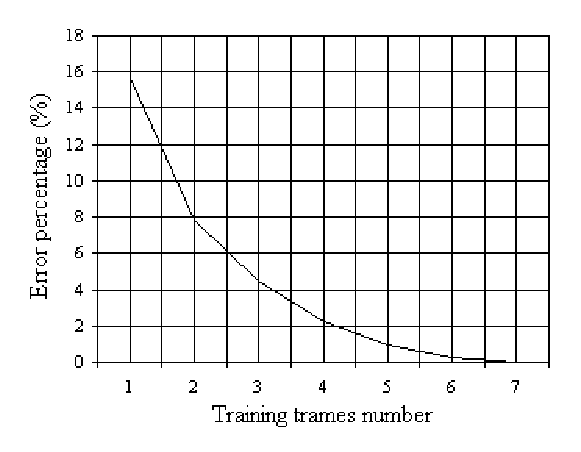
\includegraphics[width=2.7in]{Figure3}
% where an .eps filename suffix will be assumed under latex, 
% and a .pdf suffix will be assumed for pdflatex
\label{fig2b}}}
\caption{Optimal trames number in the training data set}
\label{fig2}
\end{figure}

\section{Conclusiones y Trabajos Futuros}
En este apartado se resumen las conclusiones obtenidas y se proponen futuras líneas de investigación que se deriven del trabajo.

Para añadir una referencia a un autor, se puede utilizar el paquete ''cite''. En el trabajo \cite{references:sotelo07}, se muestra un trabajo...